\chapter{Prezentacja aplikacji oraz testy}
\section{Przedstawienie aplikacji}
Użytkownik przechodząc pod adres \enquote{http://decisiontree.pl} w przeglądarce zostanie przekierowany na stronę główną projektu (Rys. \ref{rys7_home_page} ). Zobaczy tam krótki opis aplikacji. W celu korzystania z systemu wymagana jest autoryzacja użytkownika. Osoba nowa może założyć konto przy pomocy formularza rejestracji (Rys. \ref{rys8_registery_form}). Wypełniając pola użytkownik musi zaakceptować pole \enquote{\textit{recaptcha}}, pełniącą role zabezpieczenie przed botami w internecie. Po zatwierdzeniu formularza osoba zostanie automatycznie zalogowana. Użytkownicy, którzy już posiadają konto w aplikacji mogą skorzystać z pola logowania przedstawionego na Rys. \ref{rys9_login_form}.

\begin{figure}[htb]
	\centering
	\includegraphics[width=15cm]{grafika/home_page.eps}
	\caption{Strona główna aplikacji, źródło: opracowanie własne.}
	\label{rys7_home_page}
\end{figure}

\begin{figure}[htb]
	\centering
	\includegraphics[width=11cm]{grafika/registery_form.eps}
	\caption{Formularz rejestracji nowego konta, źródło: opracowanie własne.}
	\label{rys8_registery_form}
\end{figure}

\begin{figure}[htb]
	\centering
	\includegraphics[width=11cm]{grafika/login_form.eps}
	\caption{Formularz logowania, źródło: opracowanie własne.}
	\label{rys9_login_form}
\end{figure}

Uwierzytelniony użytkownik w zależności od nadanych mu uprawnień będzie miał możliwość wykonania innych akcji. Funkcje do których nie będzie miał dostępu nie będą wyświetlane w interfejsie graficznym, na przykład mając uprawnienia z poziomu \enquote{1\_default} na pasku nawigacji nie będzie zakładki \enquote{Files}. Widok przedstawiający wygląd strony dla użytkownika ze wszystkimi prawami został pokazany na Rys. \ref{rys7_home_page}. Przechodząc do zakładki \enquote{Experiments} zostanie wyświetlona lista wszystkich eksperymentów wraz z przyciskiem do tworzenia nowego doświadczenia lub podglądem już istniejącego (Rys. \ref{rys10_experiment_table}). 

Kolejnym elementem na pasku nawigacji jest odnośnik do strony zarządzania plikami użytkownika. Na tym widoku znajduję się strefa wgrywania umożliwiająca wrzucanie plików niezbędnych do przeprowadzenia doświadczenia (Rys. \ref{rys17_file_page}). W dowolnym momencie użytkownik może zmienić nazwę pliku (Rys. \ref{rys19_edit_name}), usunąć lub też pobrać dowolny plik. Podczas próby wgrania pliku o rozszerzeniu innym niż znajdujących się na liście dozwolonych dla użytkownika pojawi się ostrzeżenie o błędzie. Dodatkową funkcjonalnością jest przycisk kierujący do formularza tworzenia nowego pliku konfiguracyjnego. Formularz zawiera podstawowe pola, które są uzupełnione wartościami domyślnymi (Rys. \ref{rys18_config_form}). Stanowi to ułatwienie dla nowych użytkowników, którzy chcieliby zrobić swój pierwszy eksperyment bez zagłębiania się w zaawansowane parametry algorytmu.
\begin{figure}[htb]
	\centering
	\includegraphics[width=15cm]{grafika/experiment_table.eps}
	\caption{Widok listy eksperymentów, źródło: opracowanie własne.}
	\label{rys10_experiment_table}
\end{figure}

\begin{figure}[htb]
	\centering
	\includegraphics[height=9cm]{grafika/experiment_form.eps}
	\caption{Formularz tworzenia nowego eksperymentu, źródło: opracowanie własne.}
	\label{rys11_experiment_form}
\end{figure}



\begin{figure}[htb]
	\centering
	\includegraphics[width=15cm]{grafika/details_page.eps}
	\caption{Strona przedstawiający szczegóły eksperymentu, źródło: opracowanie własne.}
	\label{rys12_details_page}
\end{figure}

\begin{figure}[htb]
	\centering
	\includegraphics[height=11cm]{grafika/edit_experiment.eps}
	\caption{Formularz edycji eksperymentu, źródło: opracowanie własne.}
	\label{rys13_edit_experiment}
\end{figure}

\begin{figure}[htb]
	\centering
	\includegraphics[width=11cm]{grafika/share_form.eps}
	\caption{Formularz udostępniania eksperymentu, źródło: opracowanie własne.}
	\label{rys14_share_form}
\end{figure}


Proces tworzenia nowego eksperymentu rozpoczyna się od wypełnienia formularza informacjami oraz wybraniu plików wejściowych (zarówno ze zbiorami danych oraz ustawieniami algorytmu) (Rys. \ref{rys11_experiment_form}). W~przypadku niewypełnienia, któregoś pola zostanie wyświetlony komunikat o błędzie. Jeżeli wszystkie pola będą wypełnione, po zatwierdzeniu wyświetli się informacja o sukcesie oraz nastąpi przekierowanie do listy eksperymentów. Nowo stworzone doświadczenia na liście posiadają status \enquote{Created}. Klikając w przycisk \enquote{Show} użytkownik może wyświetlić szczegóły eksperymentu, wraz z listą akcji możliwych do wykonania. Po uruchomieniu doświadczenie trafia do kolejki i przyjmuje status \enquote{In queue}. Natomiast zaraz po zaczęciu obliczeń przechodzi w stan \enquote{Running} i użytkownik ma możliwość zobaczenia postępu zadania w zakładce szczegółów eksperymentu (Rys. \ref{rys15_progress_bar}). W~dowolnym czasie trwania obliczeń istnieje możliwość wysłania sygnału przerwania, wtedy status zmieni się na \enquote{Cancel}. Kiedy podczas uruchomienia wystąpi błąd oznaczenie ustawi się na wartość \enquote{Error}. W pełni ukończony eksperyment otrzymuje status \enquote{Finished}, a w widoku szczegółów pojawią się odnośniki do powstałych drzew decyzyjnych (Rys.\ref{rys12_details_page}). W~zależności od stanu doświadczenia ramka karty przyjmie inne kolory informując o rezultacie ostatnich akcji. Przechodząc do widoku z wynikami otrzymamy tabele ze statystykami takimi jak rozmiar drzewa, czas wykonania, ilość danych treningowych i~testowych poddanych ewaluacji oraz wartości procentowe rezultatów. Rysunek wynikowego drzewa można skalować przy pomocy kółka myszki, a~poszczególne węzły można zwijać i~rozwijać. Istnieje dodatkowa opcja wydrukowania wizualizacji wyników.

\begin{figure}[htb]
	\centering
	\includegraphics[width=15cm]{grafika/progress_bar.eps}
	\caption{Widok uruchomionego eksperymentu, źródło: opracowanie własne.}
	\label{rys15_progress_bar}
\end{figure}

\begin{figure}[htb]
	\centering
	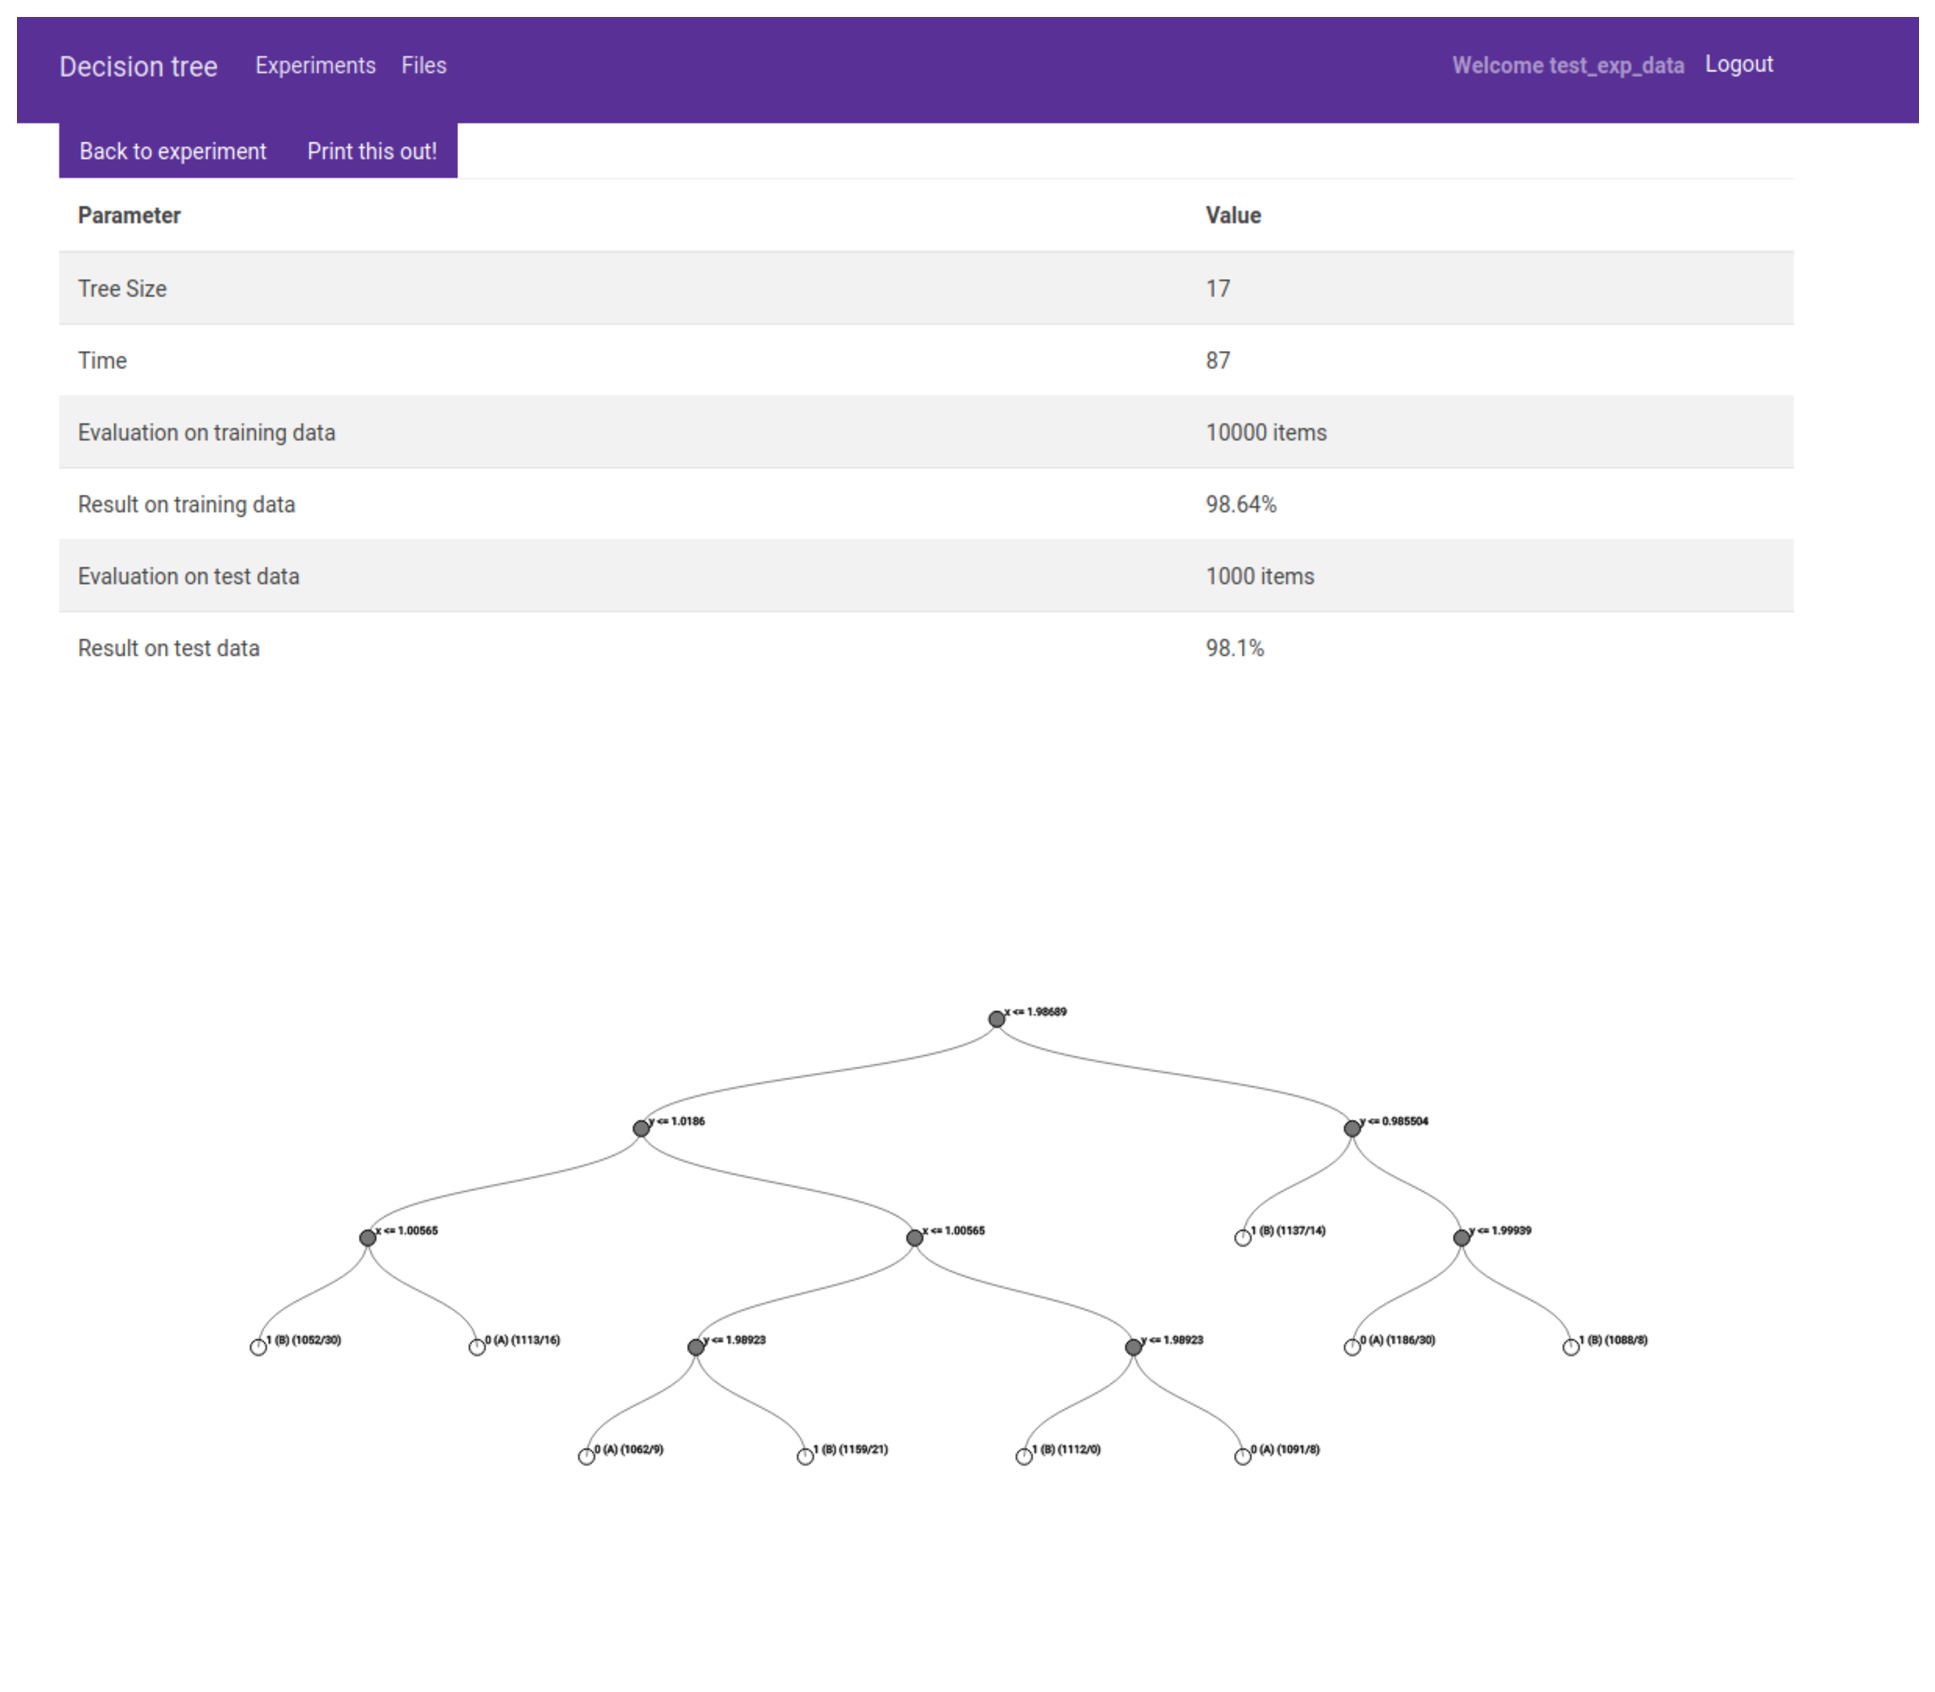
\includegraphics[width=17cm]{grafika/tree_veiw.eps}
	\caption{Widok stworzonego drzewa decyzyjnego, źródło: opracowanie własne.}
	\label{rys16_tree_veiw}
\end{figure}

\begin{figure}[htb]
	\centering
	\includegraphics[width=15cm]{grafika/tree_stat.eps}
	\caption{Tabela ze statystykami algorytmu, źródło: opracowanie własne.}
	\label{rys22_tree_stat}
\end{figure}

\begin{figure}[htb]
	\centering
	\includegraphics[width=15cm]{grafika/file_page.eps}
	\caption{Widok strony do zarządzania plikami, źródło: opracowanie własne.}
	\label{rys17_file_page}
\end{figure}

\begin{figure}[htb]
	\centering
	\includegraphics[height=10cm]{grafika/config_form.eps}
	\caption{Formularz tworzenia nowego pliku konfiguracyjnego, źródło: opracowanie własne.}
	\label{rys18_config_form}
\end{figure}

\begin{figure}[htb]
	\centering
	\includegraphics[width=9cm]{grafika/edit_name.eps}
	\caption{Formularz edycji nazwy pliku, źródło: opracowanie własne.}
	\label{rys19_edit_name}
\end{figure}

Użytkownik może wykonywać dodatkowe operacje po przez panel wyświetlenia szczegółów doświadczenia, na przykład edycję eksperymentu za pomocą formularza (Rys. \ref{rys13_edit_experiment}). Kolejną funkcjonalnością jest udostępnianie eksperymentu innym osobom. W~formularzu wyświetlają się kontrolki do nadawania praw, które zostały przedstawione na Rys. \ref{rys14_share_form}. Eksperyment po udostępnieniu pojawi się na liście wszystkich doświadczeń u~drugiej osoby. Natomiast na końcu nazwy w nawiasach zostanie dodana nazwa właściciela, który udostępnił eksperyment. 


\begin{figure}[htb]
	\centering
	\includegraphics[width=15cm]{grafika/admin_exp.eps}
	\caption{Panel modyfikacji praw dostępowych do eksperymentu, źródło: opracowanie własne.}
	\label{rys20_admin_exp}
\end{figure}

Aplikacja udostępnia również panel administratora dostępny pod adresem \enquote{decisontree.pl\textbackslash{admin}}. Po autoryzacji, administrator może zarządzać modelami w bazie, ale także zmieniać role użytkowników. Również w dowolnym momencie może modyfikować ograniczenia dostępu do eksperymentu, przez co może ograniczyć lub nadać prawa. Widok zarządzania eksperymentem został przedstawiony na Rys. \ref{rys20_admin_exp}.

\section{Testy aplikacji}
Nieodłącznym elementem związanym z tworzeniem aplikacji jest przeprowadzenie testów w celu sprawdzenia poprawności jej działania. Testowanie ma za zadanie zweryfikować czy dany produkt jest zgodny ze specyfikacją oraz wykryć błędy w kodzie. W projekcie aplikacji zostały wykorzystane testy wydajnościowe oraz manualne na grupie kontrolnej.
 
\subsection{Testy wydajnościowe}
Oprogramowaniem użytym do określenia wydajności poszczególnych punktów końcowych jest framework Locust. Narzędzie te służy do testowania obciążenia aplikacji internetowej. Głównym jego celem jest określenie maksymalnej liczby osób, które w danym czasie mogą używać aplikacja bez problemów wydajnościowych. Podczas uruchamiania zestawu testowego należy podać co ile sekund pojawi się nowy użytkownik oraz ich łączną liczbę. Na potrzeby testów aplikacji przyjęte wartości to 10, 100, 500 jednoczesnych korzystających użytkowników oraz częstotliwość tworzenia konta 10 na sekundę. Dodatkowo ten sam zestaw został uruchomiony podczas obciążenia serwera obliczeniami w systemie GDT. Wyniki poszczególnych testów zostały przedstawione w Tab. \ref{tabela_4_test_locust}. 

Analizując wartości otrzymane w testach możemy znaleźć zależność, że im większa liczba użytkowników tym dłużej serwer potrzebuje czasu na realizacje zapytania. Przy liczbie kont równej 500 pewna część żądań do aplikacji kończy się błędem oznaczającym zresetowaniem połączenia. Na podstawie wyników można określić, że liczba 100 użytkowników na raz może w dość nieograniczający sposób korzystać z aplikacji. Ograniczenia wydajnościowe są spowodowane niewielką mocą serwera. Poprawę wyników można osiągnąć poprzez zwiększenie pojemność pamięci RAM i zwiększenie mocy procesora. Jednoczesna praca nad obliczeniami powoduje spadek wydajności realizowania zapytań. Rozwiązaniem tego problemu może być opcja przeniesienia części kontenerów na oddzielne serwery. Dzięki temu moduły nie będą konkurować o moc obliczeniową.  

\begin{table}[htb]
	\caption{Wyniki testów wydajnościowych z użyciem Locust, źródło: opracowanie własne.}
	\centering
	\begin{tabular}{|c|c|c|c|p{9cm}|}
		\hline
		\textbf{Liczba użytkowników}  & \textbf{Pod obciążeniem}  & \textbf{Zapytania na sekundę} & \textbf{Średni czas odpowiedzi} \\\hline
		10 & Nie & 1.5 & 50 ms \\\hline
		100 & Nie & 15.5 & 200 ms \\\hline
		500 & Nie & 6.5 & 25000 ms \\\hline
		10 & Tak & 1.3 & 60 ms \\\hline
		100 & Tak & 8.5 & 11000 ms \\\hline
		500 & Tak & 5.0 & 35000 ms \\\hline
	
		
	\end{tabular}
	\label{tabela_4_test_locust}
\end{table}

\subsection{Testy manualne}
Testy manualne przeprowadzane zgodnie ze scenariuszami testowymi sa ważnym aspektem podczas przygotowania się do wdrożenia aplikacji. Za grupę kontrolną zostali wybrani studenci Politechniki Białystockiej. Łączna liczba osób, która wzięła udział w testach wynosiła 20. W celu przetestowania najważniejszych funkcjonalności zostały stworzone dwa zestawy testowe opisujące kolejne kroki i oczekiwane rezultaty. Przykładowy uzupełniony zestaw testowy został przedstawiony na Rys. \ref{rys21_test_case}. Jeden z nich miał za zadanie sprawdzenia następujących funkcjonalności: 
\begin{itemize}
	\item Rejestracja,
	\item Logowanie,
	\item Uruchomienie eksperymentu,
	\item Zatrzymanie doświadczenia,
	\item Ponowne uruchomienie eksperymentu,
	\item Wyświetlenie wyników.
\end{itemize}
Natomiast drugi zestaw testowy wymagał pracy w parach, a jego celem była weryfikacja: 
\begin{itemize}
 	\item Udostępnienie eksperymentu,
 	\item Uruchomienie otrzymanego doświadczenia i wyświetlenie wyników.
\end{itemize}

\begin{figure}[htb]
	\centering
	\includegraphics[width=17cm]{grafika/test_case.eps}
	\caption{Przykładowy wypełniony zestaw testowy, źródło: opracowanie własne.}
	\label{rys21_test_case}
\end{figure}

W początkowej fazie testów zostały wykryte problemy z mechanizmem kolejkowania zadań dla robotnika Celery, które zostały rozwiązane po przez zmianę konfiguracji w metodzie zadania. W kolejnych etapach nie zlokalizowano poważniejszych błędów, tylko kilka mniejszych związanych z~zachowaniem interfejsu graficznego. Wszystkie problemy, które były opisane i zweryfikowane przez grupę kontrolną zostały rozwiązane.